\documentclass[tikz,border=3pt]{standalone}
\usepackage[utf8]{inputenc}
\usepackage[T1]{fontenc}
\usepackage{lmodern}
\renewcommand{\familydefault}{\sfdefault}
\usepackage{sansmath}\sansmath
\usepackage{chemfig}
\usepackage{pgfplots}\pgfplotsset{compat=1.18,/pgf/number format/use comma,/pgf/number format/1000 sep={.}}
\usetikzlibrary{arrows.meta,calc,positioning,decorations.pathmorphing,patterns}
% paleta del sitio
\definecolor{nar}{HTML}{E8680C}\definecolor{narc}{HTML}{FFB35C}\definecolor{hielo}{HTML}{FFF3E8}
\definecolor{tinta}{HTML}{1D1D1F}\definecolor{gris}{HTML}{6E6E73}\definecolor{lila}{HTML}{7C5CF0}
\definecolor{azul}{HTML}{2F6FD6}\definecolor{menta}{HTML}{17A673}\definecolor{coral}{HTML}{E8342A}
\tikzset{cel/.style={draw=gris,fill=hielo,line width=0.9pt},nuc/.style={draw=gris!70,line width=0.6pt},
fib/.style={gris!55,line width=0.35pt},eti/.style={font=\footnotesize,text=tinta,align=center},
num/.style={circle,draw=nar,fill=white,text=nar,font=\small\bfseries,inner sep=1.2pt,minimum size=13pt},
fl/.style={-{Stealth[length=2.6mm]},gris,line width=0.9pt}}
\begin{document}
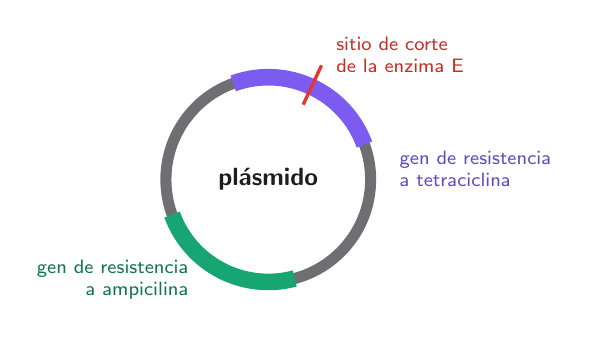
\begin{tikzpicture}[font=\small]
\draw[gris,line width=4pt] (0,0) circle (1.3);
\draw[menta,line width=6pt] (200:1.3) arc (200:285:1.3);\draw[lila,line width=6pt] (20:1.3) arc (20:110:1.3);
\draw[coral,very thick] (65:1.05)--(65:1.6);\node[font=\scriptsize,text=coral!85!black,align=left,anchor=west] at (65:1.75) {sitio de corte\\de la enzima E};
\node[font=\scriptsize,text=lila!80!black,align=left,anchor=west] at (5:1.55) {gen de resistencia\\a tetraciclina};
\node[font=\scriptsize,text=menta!70!black,align=right,anchor=east] at (235:1.55) {gen de resistencia\\a ampicilina};
\node[font=\small\bfseries,text=tinta] at (0,0) {plásmido};
\end{tikzpicture}
\end{document}
